\subsection{Kết quả}
\subsubsection{Đánh giá bằng độ đo mAP}
\begin{table}[ht]
   \begin{center}
    \caption{Kết quả mAP với threshold=0.5}
    \begin{tabular}{c | c | *3c}
    \toprule
    Mô hình &  HOG+SVM  & \multicolumn{3}{c}{Faster R-CNN}\\
    \hline
    {}   &             & lr=0.004  & lr=0.005 & lr=0.006\\
    mAP   &      0.271      & 0.591  & 0.604 & 0.619\\
    \bottomrule
    \end{tabular}
  \end{center}
\end{table}
\subsubsection{Trên tập test}
\textbf{HOG+SVM}\\

\begin{figure}[h!]
  \centering
  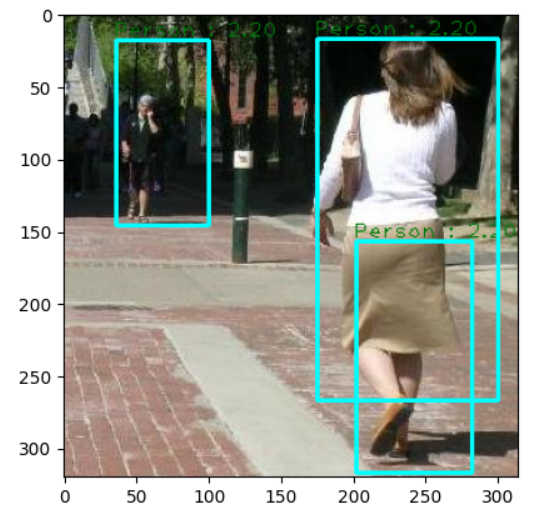
\includegraphics[scale=0.7]{graphics/testhogsvm.png}
  \caption{Kết quả mô hình HOG+SVM}
\end{figure}

Có thể thấy, HOG+SVM phát hiện người đi bộ vẫn chưa được chính xác. Một phần là vì bộ dữ liệu train model vẫn còn thấp, nhưng ta vẫn thấy được sự tương đối của mô hình này trong phát hiện đối tượng ở đây là người đi bộ.\\ 

\textbf{Faster R-CNN}
\pagebreak

\begin{figure}[h!]
  \centering
  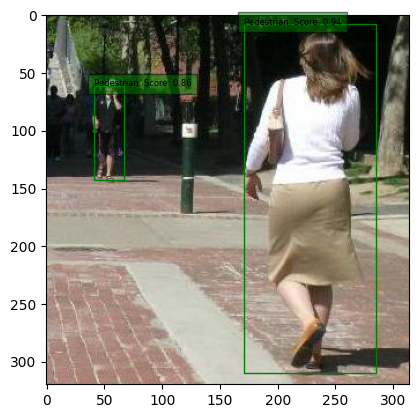
\includegraphics[scale=0.7]{graphics/test_0004.png}
  \caption{Kết quả mô hình Faster R-CNN trên tập test với r=0.004}
\end{figure}

\begin{figure}[h!]
  \centering
  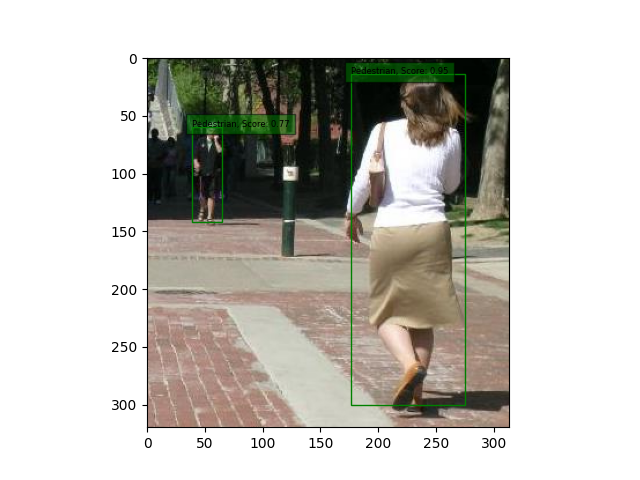
\includegraphics[scale=0.7]{graphics/test_0005.png}
  \caption{Kết quả mô hình Faster R-CNN trên tập test với lr=0.005}
\end{figure}

\pagebreak

\begin{figure}[h!]
  \centering
  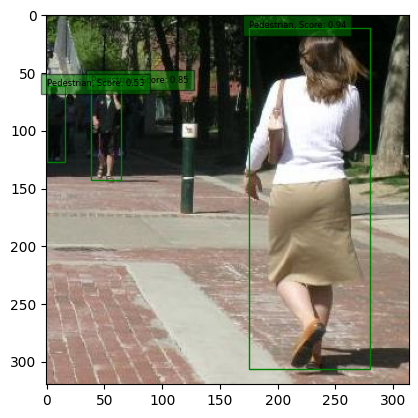
\includegraphics[scale=0.7]{graphics/test_0006.png}
  \caption{Kết quả mô hình Faster R-CNN trên tập test với lr=0.006}
\end{figure}

Theo kiến thức và thị giác của con người, ta có thể thấy rằng giữa ba giá trị của learning\_rate thì lr=0.006 cho kết quả tốt hơn so với hai giá trị còn lại vì detect được một người bị khuất trong bóng râm trong bức hình.\\

\subsubsection{Trên hình ảnh số bất kỳ}
\textbf{HOG+SVM}

\begin{figure}[h!]
  \centering
  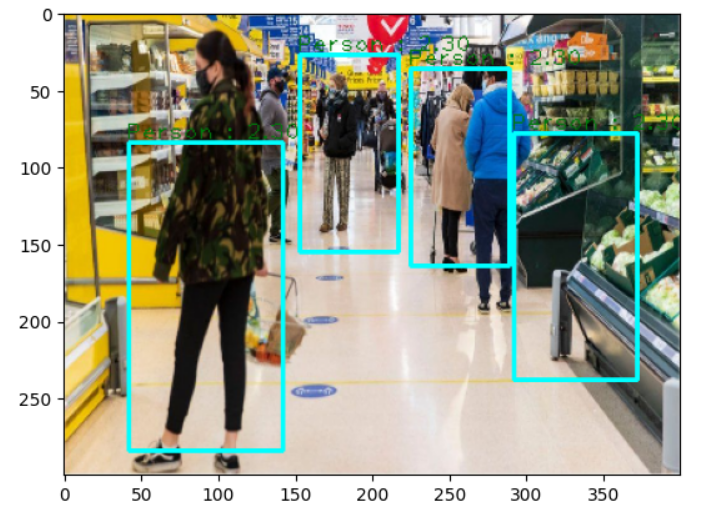
\includegraphics[scale=0.55]{graphics/rshogsvm0.png}
  \caption{Kết quả trên một hình ảnh trong siêu thị của HOG+SVM}
\end{figure}

\begin{figure}[h!]
  \centering
  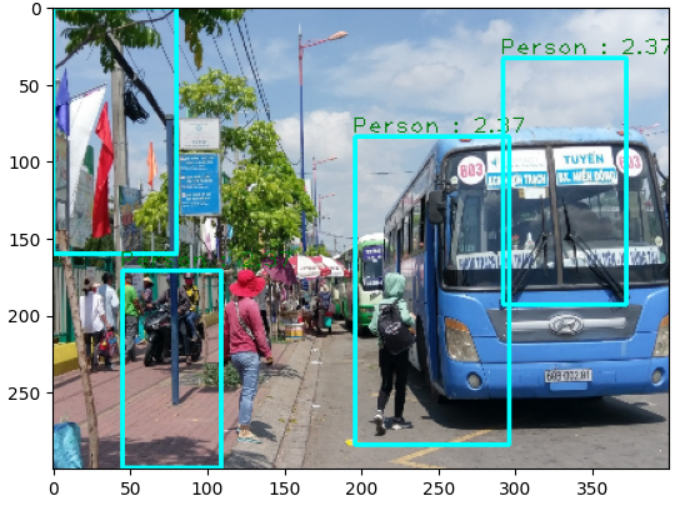
\includegraphics[scale=0.55]{graphics/rshogsvm1.png}
  \caption{Kết quả trên một hình ảnh ở bến xe buýt Suối Tiên của HOG+SVM}
\end{figure}
\pagebreak

\textbf{Faster R-CNN}

\begin{figure}[h!]
  \centering
  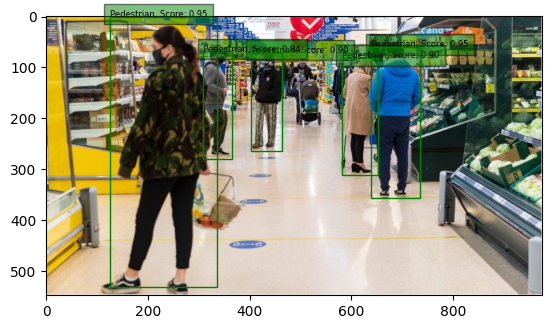
\includegraphics[scale=0.7]{graphics/demo1.png}
  \caption{Kết quả trên một hình ảnh trong siêu thị của Faster R-CNN với lr=0.006}
\end{figure}

\begin{figure}[h!]
  \centering
  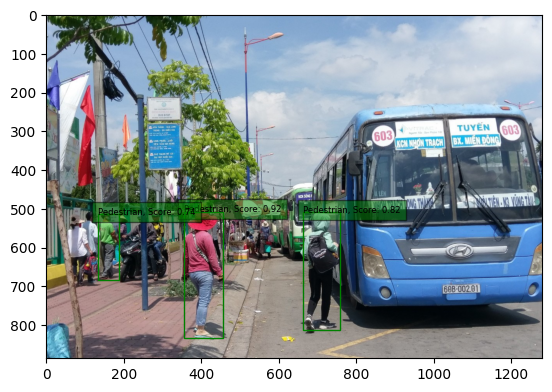
\includegraphics[scale=0.7]{graphics/demo2.png}
  \caption{Kết quả trên một hình ảnh ở bến xe buýt Suối Tiên của Faster R-CNN với lr=0.005}
\end{figure}